\section{Technische Grundlagen}
\subsection{Robotik} % Manuel ca. 8
% Farbe die angibt welchen Status der folgende Abschnitt hat:
\color{process}
% Eigentlicher Text:
Tatsächlich gibt es 
Die VDI-Richtline 2860 von 1990 definiert einen Roboter wie folgt:
\newline
>>Ein Roboter ist ein frei und wieder programmierbarer, multifunktio-
naler Manipulator mit mindestens drei unabhängigen Achsen, um Ma-
terialien, Teile, Werkzeuge oder spezielle Geräte auf programmierten,
variablen Bahnen zu bewegen zur Erfüllung der verschiedensten Auf-
gaben.<<
\newline
Auch wenn die Definition einige Eigenschaften eines Roboters ... So beschreibt diese Definition 
hauptsächlich stationäre Industrieroboter, wie sie in der Automatisierungstechnik verwendet werden,
wie beispielsweise Schweiß- oder Lackierroboter in der Automobilfertigung oder Kommissionierroboter 
in der Logistik. Die genannten programmierten Bahnen sind dort möglich und sinn-
voll, weil der Arbeitsprozess, dessen Teil der Roboter ist, gemeinsam mit dem
Roboter und seiner Programmierung gestaltet wird:
\subsubsection{Mobile Roboter}
% Farbe die angibt welchen Status der folgende Abschnitt hat:
\color{process}
% Eigentlicher Text:
Diese Kapitel ...
Anders 
\subsubsection{Sensorik}
% Farbe die angibt welchen Status der folgende Abschnitt hat:
\color{process}
% Eigentlicher Text:
Diese Kapitel ...
Sensoren lassen sich hinsichtliche ihrer Arbeitsweise und ... wie folgt klassifizieren:
\begin{itemize}
	\item{} A
	\item{} 
	\item{} 
	\item{} 
\end{itemize}
\subsubsection{Antriebsarten}
\subsection{\LM}
% Farbe die angibt welchen Status der folgende Abschnitt hat:
\color{finishing}
% Eigentlicher Text:
\LM{} ist eine seit 1988 existierende Produktserie des Spielwarenherstellers \LE{} \cite[vgl.][21]{Scholz.DasEV3}. 
\LM{} ermöglicht das Bauen, Programmieren und Steuern verschiedener \LE{} Roboter. Dies Roboter bestehen dabei aus
gängigen \LE{} Teilen die auch in anderen \LE{}-Produkten Verwendung finden, sowie speziellen \LE{}-Komponenten 
wie einer zentralen Steuereinheit, Motoren und Sensoren.
%-------------------------------------------------------------------------------------------------------------------------------------------
%### Subsektion über XXX ###################################################################################################################
%-------------------------------------------------------------------------------------------------------------------------------------------
\subsubsection{Das EV3-System}
% Farbe die angibt welchen Status der folgende Abschnitt hat:
\color{finishing}
% Eigentlicher Text:
Der 2013 erschienene EV3 ist das dritte System der \LM{} Reihe. Die Bezeichnung setzt sich aus EV für Evolution 
und 3 für die 3 Stufe der \LM{}-Serie zusammen \cite[vgl.][Seite 21]{Scholz.DasEV3}. \\
Im Vergleich zu den Vorgängersystemen verfügt das EV3-System über eine modernere und leistungsfähigere Steuereinheit und auch die anderen elektronischen Komponenten des System wurden an den heutigen Stand der Technik 
angepasst \cite[vgl.][Seite 22]{Scholz.DasEV3}.
\medskip
\newline
Die folgende Abbildung X.X zeigt einige der zentralen Komponeten des EV3-Systems, wie die Steuereinheit (EV3-Stein), Motoren und vier Sensoren.
\begin{figure}[ht]
	\centering
	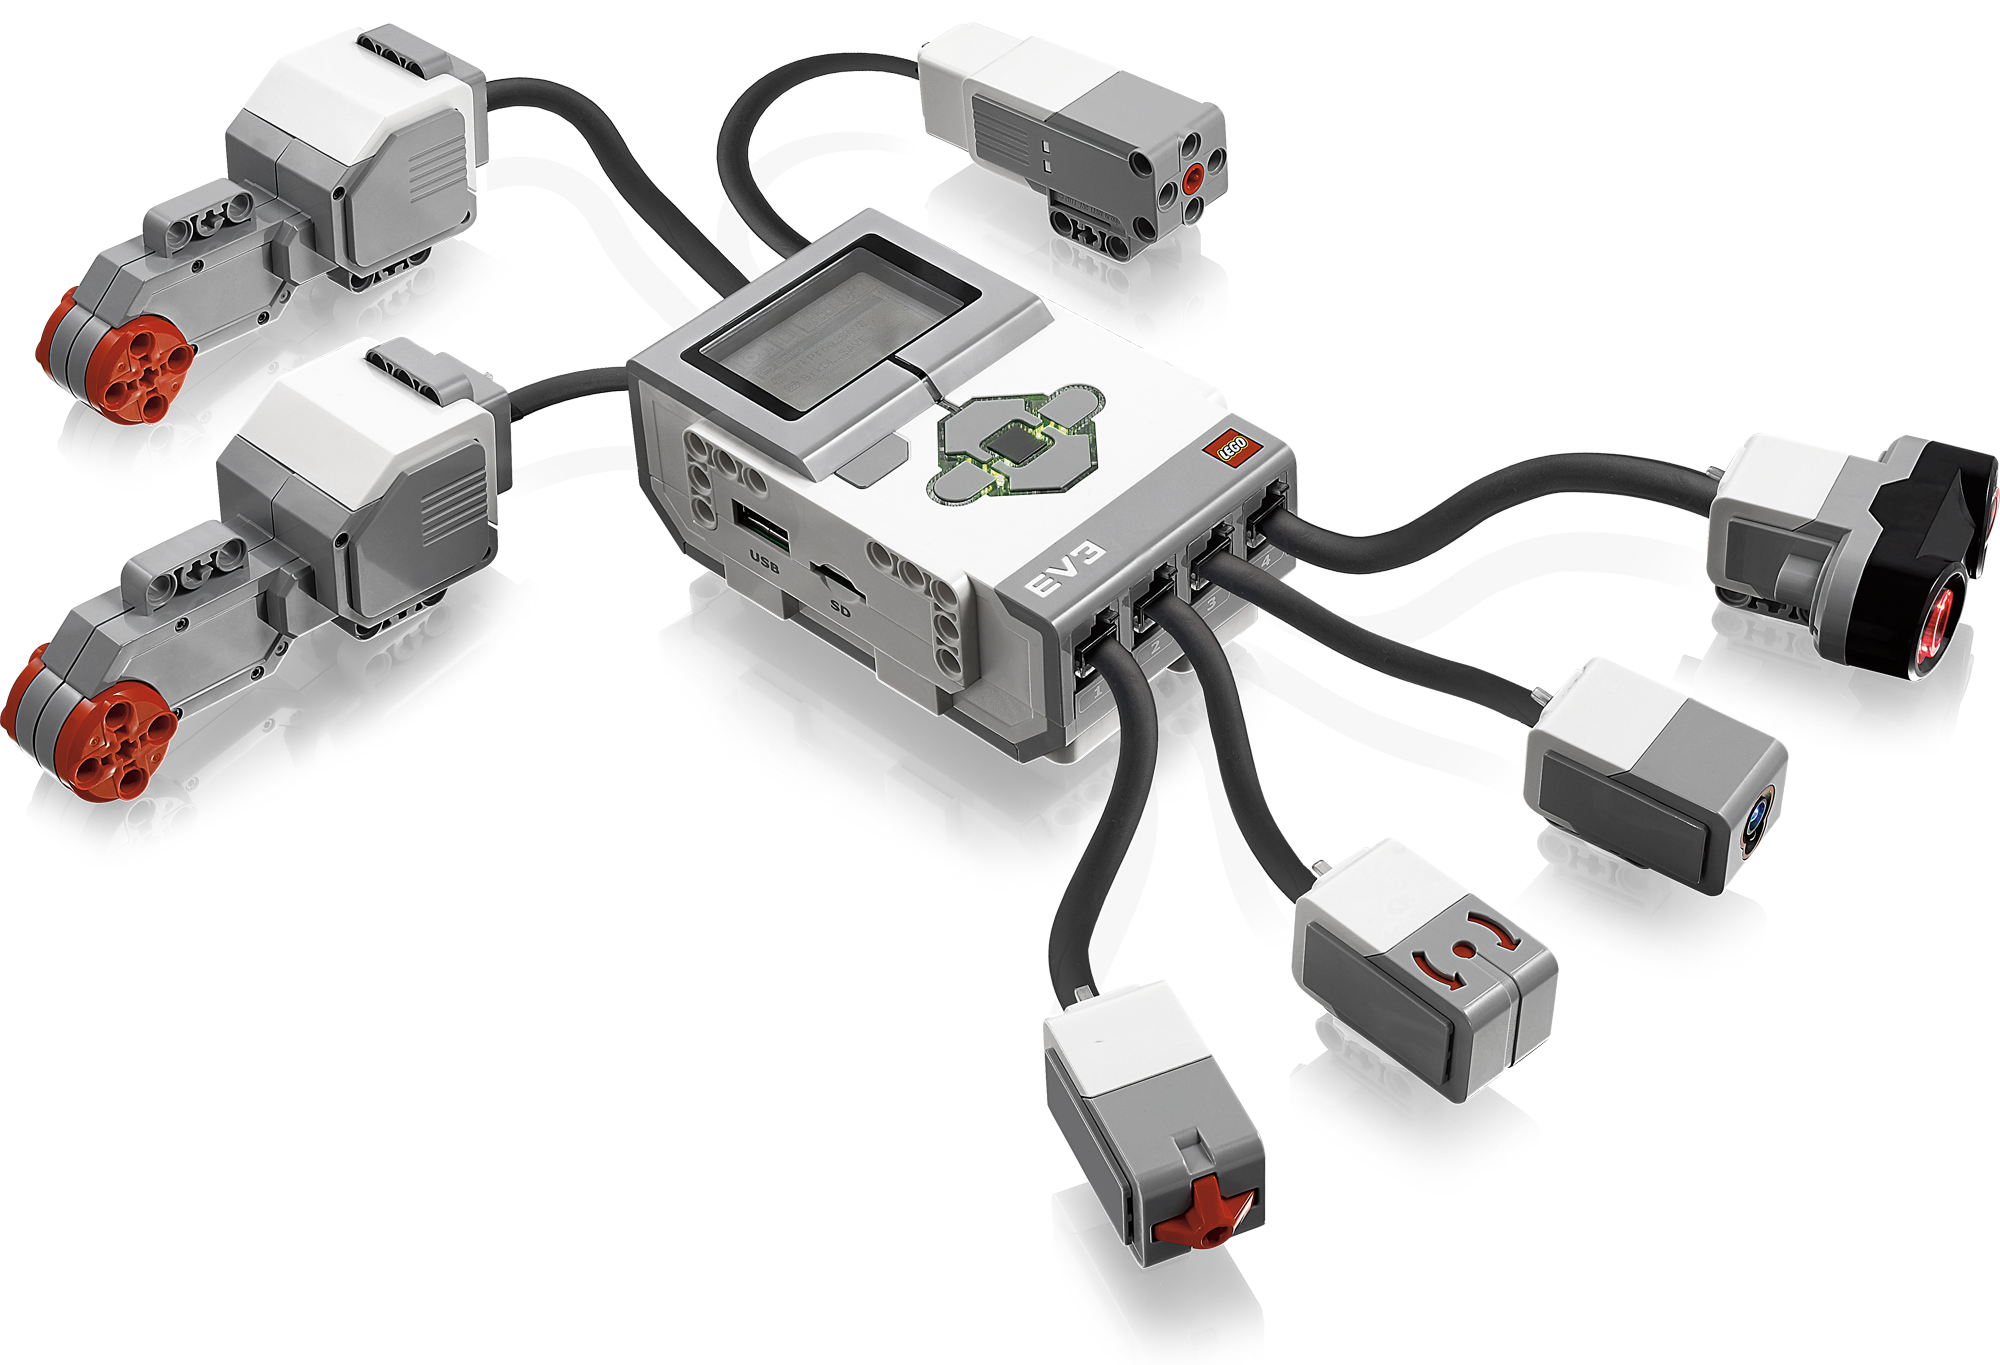
\includegraphics[width=0.90\textwidth]{images/technische_grundlagen/EV3-Overview.png}
	\caption[Zentrale Komponenten des EV3-Systems]{Zentrale Komponenten des EV3-Systems}
	\label{fig:<Sprungmakre>}
\end{figure}
\newline
Neben den elektronischen Komponeten gehören auch nicht elektronische Teile wie Verbindungsstücke, Balken und Zahnräder 
wie sie aus gängigen \LE{} Produkten bekannt sind, zum EV3-System. Sie bilden die strukturelle und meschanische Grundlage 
der Roboter.
\medskip
\newline
Im Folgenden wird auf die elektronischen Komponenten des EV3-Systems näher eingegangen.
dieses Projekt eine deutlich größere Relevanzu aufweisen.
\subsubsection{Der EV3-Stein (Steuereinheit)}
% Farbe die angibt welchen Status der folgende Abschnitt hat:
\color{finishing}
% Eigentlicher Text:
Die zentrale Komponenten und das Gehirn des LEGO MINDSTORMS EV3-Systems ist die zentrale Steuereinheit kurz (EV3-)Stein oder auch Brick genannt. Bei ihm handelt
es sich um eine Computer welcher selbständig Programme ausführen kann. Dazu verfügt der EV3-Stein über 
ein Linux Betriebssystem und eine spezielle Firmware, die wie die auszuführenden Programme auf einem Flash-Speicher liegen \cite[vgl.][21]{Scholz.DasEV3}. \\
Zur Kommunikation mit dem PC verfügt der EV3-Stein über eine USB- sowie Bluetooth-Schnittstelle. Neben der 
Kommunikation zu einem Computer kann die USB-Schnittstelle auch für den Zusammenschluss mit einem weiteren EV3-Stein (genannt Daisy Chain) 
genutzt werden \cite[vgl.][Seite 21]{Scholz.DasEV3}.  \\
Für den Anschluss von Motoren und Sensoren verfügt der EV3-Stein über 8 Ports, an welche die anderen System-Komponenten müber Kabel mit RJ12-Steckern angeschlossen werden. 4 der Ports dienen für den Anschluss von
Motoren, die restlichen 4 Ports für die Abfrage von Sensorwerte \cite[vgl.][21]{Scholz.DasEV3}.  \\
Der EV3-Stein besitzt an der Vorderseite ein LCD-Display zur Anzeige von Texten und Grafiken sowie  
6 Knöpfe für die Bedienung durch den Benutzer. Display und Knöpfe dienen zur Bedienung der Firmware sowie zur Tätigung von Einstellungen, können aber ebenso durch Programmen angesprochen und ausgewertet werden
Start
Mein Kanal
Trends
Abos
BIBLIOTHEK
\cite[vgl.][21]{Scholz.DasEV3}. 
\smallskip
\newline
Die folgende Auflistung zeigt einige Leistungsmerkmale des EV3-Steins \citep[vgl.][Seite 23 f., Seite 32]{Scholz.DasEV3, Schobel.RobertaEV3Programmieren}.
\begin{itemize}
	\item{Prozessor:} ARM9 32Bit, 300 MHz, 16 MB Flash 64MB RAM
	\item{Betriebssystem:} Linux
	\item{Sensoranschlüsse:} 4x, Analog / Digital bis zu 460,8 Kbit/s
	\item{USB-Schnittstellen:} 2x, für Kommunikation zum PC, Daisy Chain, WiFi-Stick, USB-Speichermedium
	\item{SD-Karten-Lesegerät:} 1x, für MicroSD-Karte bis 32 GB
	\item{User-Interface:} 6 Knöpfe inkl. Beleuchtung
	\item{Display:} LCD Matrix, monochrom, 178 x 128 Pixel
	\item{Kommunikation:} Bluetooth v2.1, USB 2.0 (Kommunikation zum PC), USB 1.1 (Daisy Chain)
\end{itemize}
\subsubsection{Motoren}
% Farbe die angibt welchen Status der folgende Abschnitt hat:
\color{finishing}
% Eigentlicher Text:
Das EV3-System verfügt über zwei unterschiedliche Motoren, einen großen Motor und einen mittleren Motor. 
Bei beiden handelt es sich um Servormotoren mit integriertem Rotationssensor, welche von außen angesteuert und abgefragt werden können \cite[vgl.][92]{Schobel.RobertaEV3Programmieren}. Die Motoren lassen sich sehr exakt steuern und ermöglichen so einen synchronen Betrieb mehrerer Motoren \cite[vgl.][Seite 29 f.]{Scholz.DasEV3}.
\smallskip
\newline
Die folgende Tabelle zeigt die wichtigsten Eigenschaften der beiden Motoren.
\begin{table}[ht]
	\begin{tabular}{|p{4,5cm}|p{4,0cm}|p{4,0cm}|} \hline
		Eigenschaft / Motortyp		                & Großer Motor         & Mittlerer Motor    \\ \hline
		Winkelgenauigkeit       & 1 $^\circ$           & 1 $^\circ$         \\ \hline
		Umdrehungen    			& 160 bis 170 U/min    & 240 bis 250 U/min  \\ \hline 
		Drehmoment Rotation		& 20 Ncm               & 8 Ncm    			\\ \hline  
		Drehmoment Stillstand 	& 40 Ncm               & 12 Ncm    			\\ \hline  
		Gewicht    				& 76g                  & 36g   		 		\\ \hline
	\end{tabular}
	\centering
	\caption[Eigenschaften der EV3-Motortypen]{Eigenschaften der EV3-Motoren}
\end{table}
\subsubsection{Sensoren}
% Farbe die angibt welchen Status der folgende Abschnitt hat:
\color{finishing}
% Eigentlicher Text:
Zum EV3-System gehören eine Reihe von verschiedenen Sensoren die es den Robotern ermöglichen Informationen über ihre Umwelt zu sammeln sowie ihre Eigenbewegungen zu erfassen. Im folgenden Abschnitt werden die wichtigsten Sensoren mit ihren Leistungsmerkmalen beschrieben.
\paragraph{Farbsensor}
% Farbe die angibt welchen Status der folgende Abschnitt hat:
\color{finishing}
% Eigentlicher Text:
Der Frabsensor ist ein digitaler Sensor der dazu dient die Lichtintensität sowie verschiedener Farben zu erkennen. Der Sensor kann sowohl
aktiv als auch passiv betrieben werden und verfügt dafür über vier unterschiedliche Betriebsmodi  \cite[vgl.][101]{Schobel.RobertaEV3Programmieren}:
\begin{itemize}
	\item{Farbmodus (passiv)} - In diesem Modus erkennt der Sensor 7 verschiedenen Farben.
	\item{RGB-Modus (aktiv)} - In diesem Modus sendet der Sensor nacheinander rotes, grünes und balues Licht aus, je nachdem zu welchem Anteil ein Gegenstand die einzelnen Farben reflektiert wird die Frabe des Gegenstands ermittelt.
	\item{Rotlicht-Modus (aktiv)} - Bei diesem Modus wird Rotlicht ausgesendet und die Intensität des reflektierten Lichts gemessen.
	\item{Umgebungslicht-Modus (passiv)} - Bei diesem Modus wird die Intesnsität des in das Sensorfenster eindringende Umgebungslichts gemessen.
\end{itemize}
\smallskip
Eigenschaften:
\begin{itemize}
	\item{Erkennung der Farben:} keine Farbe, Schwarz, Blau, Grün, Gelb, Rot, Weiß, Barun
	\item{Abtastrate:} 1.000 Hz
	\item{Entfrenung:} 15 bis 50 mm
\end{itemize}
Durch diesen Sensor wird es beispielsweise möglich den Roboter einer frabigen Linie auf dem Boden zu folgen.
\paragraph{Ultraschallsensor}
% Farbe die angibt welchen Status der folgende Abschnitt hat:
\color{finishing}
% Eigentlicher Text:
Diese aktive Sensor verwendet für den Menschen unhörbaren Ultraschall um die Entfernung von Objekten zu ermitteln.
Der Sensor emmitiert dazu Untraschall und misst die Laufzeit der Schallwellen, wenn diese von einem Objekt reflektiert
werden, aus der Laufzeit kann dann die Entfernung ermittelt werden.
Der Senors verfügt über zwei unterschiedliche Betriebsmodi \cite[vgl.][32 f.]{Scholz.DasEV3}:
\begin{itemize}
	\item{Messen} - In diesem Modus sendet der Sensor Ultraschall aus um die Entfernung von Objekten zu ermitteln.
	\item{Scannen} - In diesem passiven Modus emittiert der Sensor selbst keinen Untraschall, sondern er reagiert auf >>fremden<< Ultraschall und kann so einen anderen aktiven Ultraschallsensor erkennen.
\end{itemize}
\smallskip
Eigenschaften:
\begin{itemize}
	\item{Genauigkeit: +/- 1 cm}
	\item{Messbereich: 3 cm bis 250 cm}
\end{itemize}
\paragraph{Berührungssensor}
% Farbe die angibt welchen Status der folgende Abschnitt hat:
\color{finishing}
% Eigentlicher Text:
Der Berührungssensor ist ein einfacher mechanischer Sensor. Wird der Knopf am Ende des Senors gedrückt wird dies
registriert. Trotz der Einfachheit dieses Sensors ist dieser dennoch sehr nützlich, da er beispielsweise die
Kollision des Roboters mit einem Hindernis erkennen kann \cite[vgl.][33]{Scholz.DasEV3}.
\paragraph{Kreiselsensor (Gyroskop)}
% Farbe die angibt welchen Status der folgende Abschnitt hat:
\color{finishing}
% Eigentlicher Text:
Der Kreiselsensor ermöglicht es Drehbewegungen um eine Achse über Rotationsgeschwindigkeit und Drehwinkel zu 
messen. Dadurch wird es möglich die Eigenbewegung des Roboters oder einer Roboterkomponente zu registrieren 
\cite[vgl.][33]{Scholz.DasEV3}.
\medskip
\newline
Eigenschaften:
\begin{itemize}
	\item{Genauigkeit: +/- 3$^\circ$ (bei einer 90$^\circ$ Drehung)}
	\item{Geschwindigkeit: maximal 440 Grad/Sekunde}
	\item{Abtastrate: 1.000 Hz}
\end{itemize}
\paragraph{Rotationssensor (Integiert)}
% Farbe die angibt welchen Status der folgende Abschnitt hat:
\color{finishing}
% Eigentlicher Text:
Wie bereits im Abschnitt X.X dargelegt verfügen die beiden Motortypen über initgrierte Rotationssensoren die es
ermöglichen, die Umdrehungen der Motoren auszulesen. Durch diese Sensoren ist es möglich durch Odometrie 
Rückschlüsse über die Bewegung bzw. Position des Roboters zu schließen.
\medskip
\newline
Eigenschaften:
\begin{itemize}
	\item{Genauigkeit: 1$^\circ$ }
	\item{Umdrehungen: Motorabhängig}
\end{itemize}
\bigskip
Neben den hier vorgestellten Sensoren existiert noch ein Infrarotsensor, welcher in Verbindung mit einer Infrarotfernsteruerung dazu dient einen EV3-Roboter fernzusteuern.
%### Subsubsektion über XXX ################################################################################################################
\subsubsection{Programmierung}
% Farbe die angibt welchen Status der folgende Abschnitt hat:
\color{process}
% Eigentlicher Text:
Für die Programmierung der \LM{} Produkte gibt es eine Reihe unterschiedlicher Programmiersprachen und -umgebungen. Die hauseigene \LE{}-Software zur Programmierung des EV3 richtet sich an Einsteiger. Sie ermöglicht es über eine grafische Oberfläche via vorgefertigter Programmabläufe welche durch grafische Blöcke repräsentiert werden den EV3 zu programmieren.\footnote{\citep[vgl.][25 f.]{Schobel.RobertaEV3Programmieren}\label{Roberta25psq}} \\
%cite[vgl.][25\psq]{Roberta}.
Die Abbildung X.X gibt einen Überblick über verschiedene für den EV3 verfügbare Programmiersprechen sowie ihre Vor- und Nachteile.
\paragraph{leJOS}
Das LEGO Java Operating System abgekürzt leJOS ist ein Framework, das es ermöglicht den EV3 mit der Programmiersprache Java zu programmieren. Das leJOS-Projekt wurde 1999 gegründet und sämtliche Komponenten (wie auch Java) sind kostenlos verfügbar \cite[vgl.][21 f.]{Schobel.RobertaEV3Programmieren}. \\
leJOS bietet eine schlanke Java Virtual Machine (JVM) für den EV3-Stein sowie eine Klassenbibliothek mit welcher die Komponenten des EV3 (Motoren, Sensoren etc.) angesprochen werden können. Installiert wird leJOS auf einer bootbaren microSD-Karte und kann anschließend davon gestartet werden, ohne die auf dem EV3 vorhandene LEGO-Software zu löschen oder zu verändern \cite[vgl.][23 f.]{Schobel.RobertaEV3Programmieren}. \\
Durch leJOS ist es möglich den EV3 mit Hilfe der Hochsprache Java zu programmieren womit eine mächtige
Programmiersprache zur Verfügung steht und die Vorteile der Objektorientierung für den EV3 genutzt werden können.
\begin{table}[ht]
	\begin{tabular}{|p{4,5cm}|p{2,0cm}|p{2,0cm}|p{2,0cm}|p{2,0cm}|} \hline
		Eigenschaft / Programmiersprache  & leJOS      & EV3-Software  & RobotC  & NEPO       \\ \hline
		Installation                      & +          & ++            & +       & +++        \\ \hline
		Handhabung    		           	  & +          & ++            & +       & ++         \\ \hline
		Kosten                            & kostenlos  & kostenlos     & 49\$    & kostenlos  \\ \hline
		Einstieg 	                      & 0          & ++            & +       & +++        \\ \hline  
		Funktionsumfang    				  & ++         & +             & ++      & ++         \\ \hline
	\end{tabular}
	\centering
	\newline
	0 = neutral; + = gut; ++ = sehr gut; +++ = hervorragend
	\caption[Eigenschaften der EV3-Motortypen]{Eigenschaften der EV3-Motoren}
\end{table}
leJOS bietet eine umfangreiche Klassenbibliothek sowie gut dokumentierte API was unter anderem die
Integration von weiteren Sensoren etc. erleichter \cite[vgl.][23 f.]{Schobel.RobertaEV3Programmieren}.
Im folgenden sind einige Features die leJOS bietet aufgelistet:
\begin{itemize}
	\item{Objektorientierte Programmierung mit Java}
	\item{Die meisten Klassen der Pakete \code{java.lang}, \code{java.util} und \code{java.io}}
	\item{Rekursion}
	\item{Synchronisation}
	\item{Multithreading}
	\item{Exceptions}
	\item{Vollständige Bluetooth unterstützung}
	\item{Unfangreiche Klassenbibliothek zum Steuern und Auslesen der EV3-Komponeten}
	\item{High-Level-Robotik-Tasks (Navigation, Localization etc.)}
\end{itemize}

\newpage
\color{finishing}
\subsection{\gls{app} Entwicklung} %Simon ca. 8

\begin{wrapfigure}{r}{0.45\textwidth}
	\begin{center}
		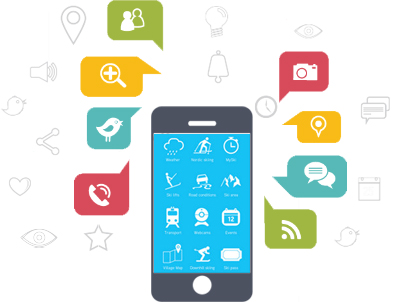
\includegraphics[width=0.4\textwidth]{images/technische_grundlagen/App-Development.jpg}
	\end{center}
	\caption{App Entwicklung}
	\label{fig:appentwicklung}
\end{wrapfigure}

Eine \gls{app} ist ein ausführbares Programm für mobile Geräte, wie Smartphones oder Tablets. Um eine \gls{app} für ein mobiles Gerät zu entwickeln, müssen wie für andere Anwendungen im Voraus Anforderungen definiert werden, die diese erfüllen soll. Je nach festgelegten Anforderungen, die an das System gestellt werden, besteht eine bestimmte Anzahl von Möglichkeiten der Entwicklung. Allgemein kennt die \gls{app} Entwicklung drei verschiedene Arten, die native, web und hybride Entwicklung, siehe \eqref{native}, \eqref{web} und \eqref{hybride}. Dabei werden verschiedene \glspl{framework} verwendet, um mit unterschiedlichsten Programmiersprachen den Aufbau der Logik zu beschreiben. Eine App besteht immer aus zwei Teile, dem \gls{ui}, das meist mit einer \gls{xml} ähnlichen Sprache beschrieben wird und dem Programmcode, der sich auf viele Klassen verteilt und die Funktionalitäten der \gls{app} beschreiben.

\subsubsection{Native \glspl{app}}\label{native}

In der Entwicklung von nativen \glspl{app} werden die direkten Ressourcen des Gerätes verwendet. Dazu gehört die Laufzeitumgebung des Betriebssystemes, Bibliotheken und Hardwareschnittstellen. Der Vorteil von einer nativen Entwicklung liegt hauptsächlich darin, dass diese für das Betriebssystem optimiert ist und die vorhandenen Schnittstellen genutzt werden können, um komplexe und rechenintensive Anwendungen zu ermöglichen.\footnote{\citep[vgl.][Unterschiede und Vergleich native Apps vs. Web Apps]{DanielWurstl.Unterschiedeund}\label{note1}}\\
Vertreter diese Entwicklung finden sich für verschiedene Betriebssysteme. Der populärste unter ihnen ist bei weitem Android mit einer nativen Java Entwicklung über Android Studio von Google. Sie besitzt aktuellen den höchsten Marktanteil und eine entsprechende Popularität unter Entwickler und Nutzer.

\subsubsection{Web \glspl{app}}\label{web}

Die Entwicklung von web \glspl{app} arbeitet mit systemübergreifenden Ressourcen und greift auf gängige Webtechnologien, wie \gls{html}, \gls{css} und \gls{javascript} zurück. Die \gls{app} wird hierbei nicht wie normale Anwendungen direkt auf dem System des Gerätes ausgeführt, sondern kommt in dessen Browser zur Ausführung. Der Vorteil hierbei ist vor allem, dass diese Art von \gls{app} auf allen Betriebssystemen lauffähig ist und direkt über das Internet veröffentlicht und aktualisiert werden kann, jedoch wird eine stabile Internetverbindung vorausgesetzt.\footref{note1}\\
Von dieser Entwicklung finden sich viele Vertreter mit der Unterstützung diverser \glspl{framework}. Das populärste unter ihnen ist aktuell AngularJS von Google, was auf \gls{javascript} basiert. In Kombination mit anderen Webtechnologien, wie \gls{html} und \gls{css} lassen sich perfomante web \glspl{app} entwickeln.

\subsubsection{Hybride \glspl{app}}\label{hybride}

Die Entwicklung von hybride \glspl{app} vereinigt die beiden Entwicklungen von native und web. Sie besteht dabei aus einem nativen Rahmen, in der eine web \gls{app} zur Ausführung kommt, diese besitzt entsprechende Zugriffsrechte auf Hardwareschnittstellen, um diese mit \glspl{api} anzusprechen.\footnote{\citep[vgl.][Native App, Web App und Hybrid App im Überblick]{PetraRiepe.NativeApp}\label{note2}}\\
Diese Entwicklung ist aktuell noch sehr jung, jedoch stechen hier bereits verschiedene Vertreter hervor. Der populärste unter ihnen ist Ionic von Drifty, welches auf Apache Cordova als Basis zurückgreift. In Kombination mit AngularJS, \gls{typescript} und anderen Webtechnologien lässt sich die web \gls{app} entwickeln und auf einem beliebigen Gerät unter einem nativen Browser ausführen. Es unterstützt dabei verschiedenste Betriebssystem, wie Android, iOS und Windows. Diese Entwicklungen können dabei meist nicht nur mobil, sondern unter anderem auf weiteren Systemen, wie stationäre bereitgestellt werden.

\subsubsection{Plattformübergreifende Entwicklung}

Um die Entwicklung von \glspl{app} einfach zu halten, verwenden immer mehr Entwickler die Form der plattformübergreifenden Entwicklung. Dadurch lässt sich die \gls{app} unabhängig des Betriebssystems entwickeln und kann somit eine größere Menge von Nutzern erreichen. Diese Entwicklung greift dabei meist auf plattformübergreifende Konzepte, wie eine native Laufzeitumgebung, oder Browser zurück, um darin die \gls{app} auszuführen. Der große Vorteil in dieser Entwicklung, liegt in der Wiederverwendbarkeit des Quellcodes und der verbesserten Wartbarkeit, da hier lediglich ein Projekt gewartet werden muss und der Quellcode für viele Betriebssysteme übernommen werden kann. Zur plattformübergreifenden Entwicklung wurden die letzten Jahre viele Ansätze mit verschiedenen \glspl{framework} entwickelt. Beispiele hierfür sind Ionic, Unity, Qt oder Xamarin.\\
\newpage

\color{process}
\subsubsection{Xamarin}

\begin{wrapfigure}{r}{0.3\textwidth}
	\begin{center}
		
\includegraphics[width=0.25\textwidth]{images/technische_grundlagen/xamarin.png}
	\end{center}
	\caption{Xamarin}
	\label{fig:xamarin}
\end{wrapfigure}

Xamarin ist ein \gls{framework} zur Entwicklung von nativen plattformübergreifenden Apps, welches auf Mono basiert, siehe \eqref{mono}. Um nativen Quellcode auf den verschiedenen Systemen auszuführen, setzt Xamarin auf verschiedene Softwarekomponenten, um aus einem mit .NET entwickelten Projekt nativen Quellcode zu erzeugen.\\
Für iOS Systeme verwendet Xamarin den \gls{aot} Compiler, um aus einem Xamarin.iOS Projekt \gls{arm} Maschinencode zur erzeugen, der entsprechend schnell auf dem System ausgeführt werden kann.\footnote{\citep[vgl.][Introduction to Mobile Development - Xamarin]{Xamarin.Introductionto}\label{note3}} Bei Android hingegen wird der Quellcode in \gls{il} übersetzt, welches \gls{jit} nutzt um zur Laufzeit Maschinencode für das entsprechende Gerät zu erzeugen.\footref{note3} Dazu nutzt Xamarin Softwarekomponenten, während der Laufzeit, um bestimmte Prozesse, wie Speicherverwaltung und Plattformoperationen. Zur Entwicklung bringt Xamarin eine große Bandbreite von Funktionalitäten für den Entwickler, wie Bibliotheken, eine Test Cloud, sowie Unterstützung von nativen Bibliotheken, wie für \gls{java} oder \gls{objectivc}. Xamarin bietet Unterstützung für diverse Betriebssysteme, wie zum Beispiel Android, iOS, Windows und Windows Phone. Um mit Xamarin zu entwickeln, gibt es aktuell verschiedene Möglichkeiten mit Unterstützung auf unterschiedlichen Betriebssystemen. Einerseits kann mit Xamarin Studio auf einem OSX System, oder mit Visual Studio auf Windows und Linux entwickelt werden.\\
Wie viele andere \glspl{framework}, bietet auch Xamarin verschiedene nützliche \glspl{template}, die jeweils andere Nutzen besitzen. Diese bauen dabei auf zwei Hauptkomponenten von Bibliotheken, einerseits Shared Projects und Protable Class Libraries.

\begin{wrapfigure}{r}{0.65\textwidth}
	\begin{center}
		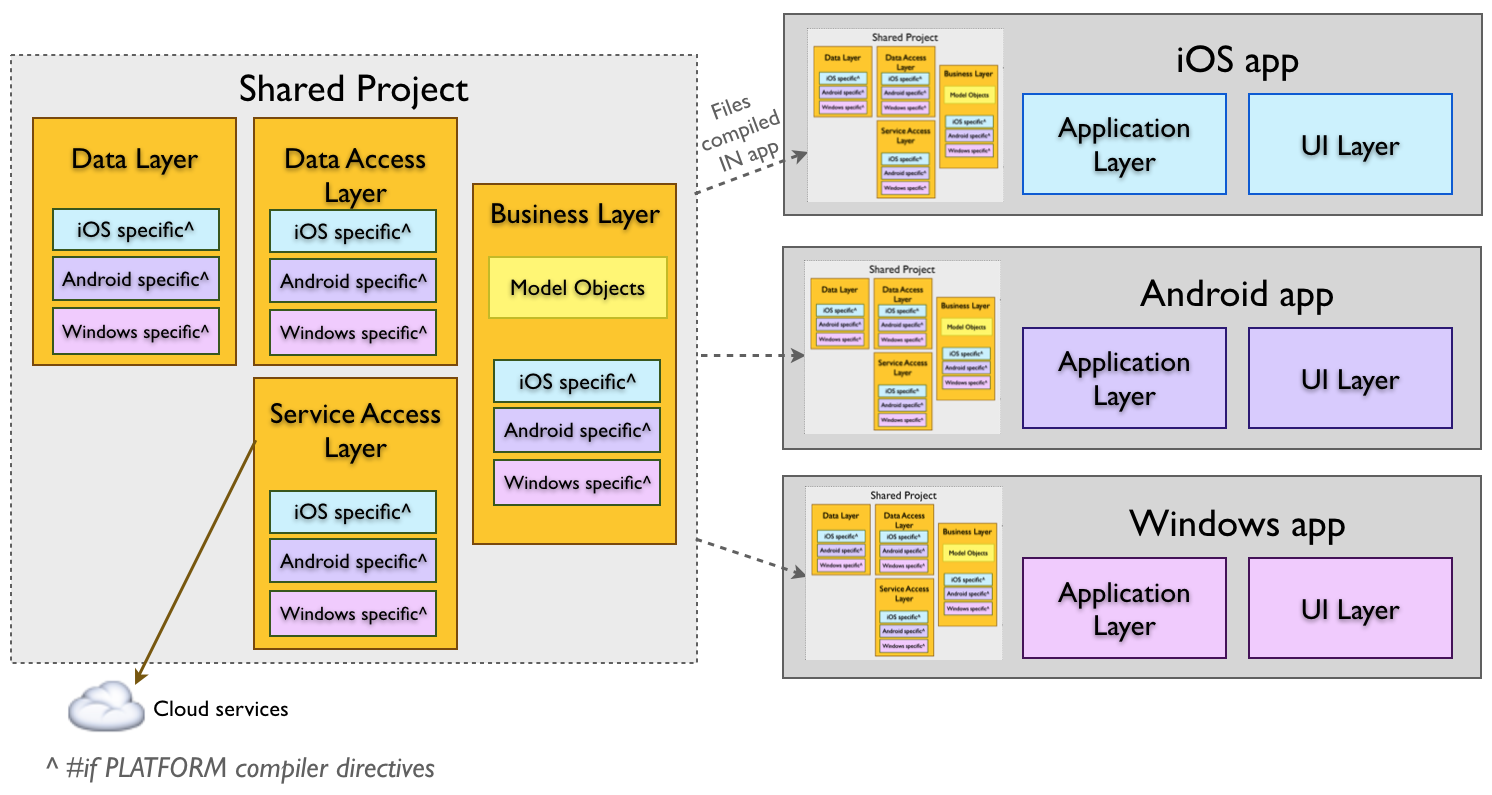
\includegraphics[width=0.6\textwidth]{images/technische_grundlagen/SharedAssetProject.png}
	\end{center}
	\caption{Shared Project}
	\label{fig:xamarin}
\end{wrapfigure}

\paragraph{Shared Projects}


, welches die Möglichkeit bietet den erstellten Quellcode für verschiedene Systeme bereitzustellen und in andere Projekte, wie Xamarin native Projekte bereitzustellen.

\begin{wrapfigure}{r}{0.65\textwidth}
	\begin{center}
		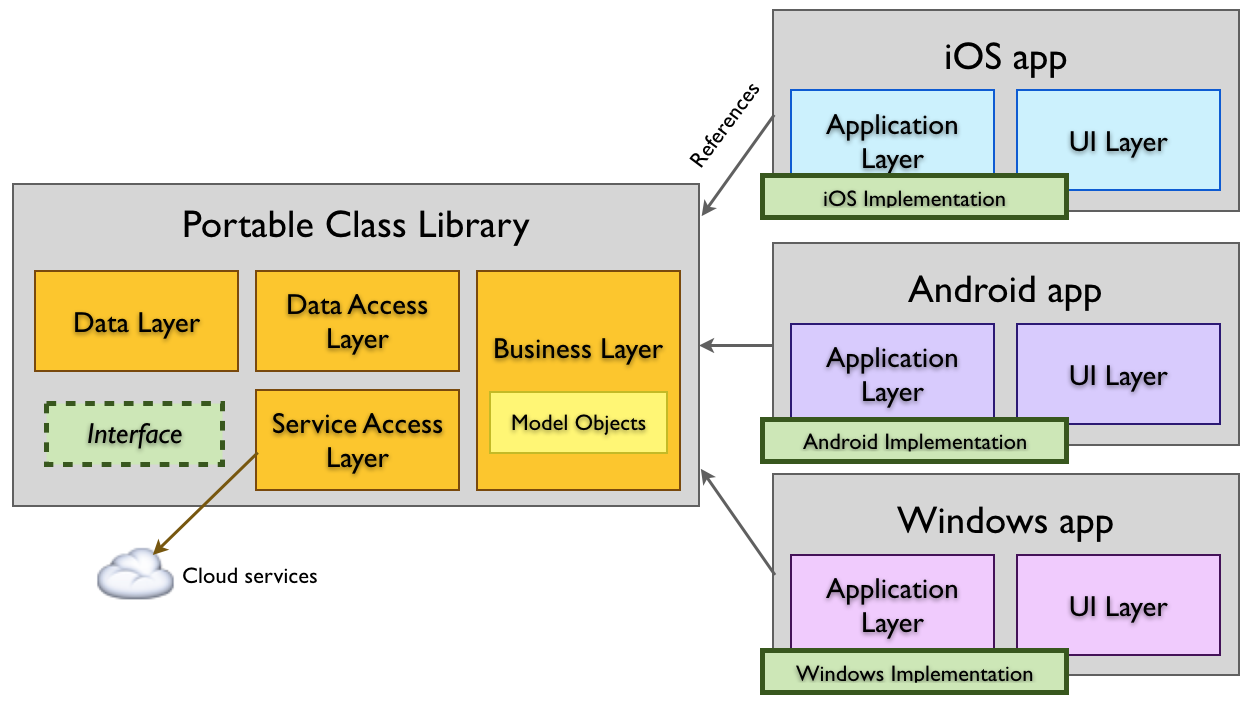
\includegraphics[width=0.6\textwidth]{images/technische_grundlagen/PortableClassLibrary.png}
	\end{center}
	\caption{Portable Class Library}
	\label{fig:xamarin}
\end{wrapfigure}

\paragraph{Protable Class Libraries}



\subsubsection{Mono}\label{mono}

\begin{wrapfigure}{r}{0.3\textwidth}
	\begin{center}
		
\includegraphics[width=0.25\textwidth]{images/technische_grundlagen/mono.png}
	\end{center}
	\caption{Mono}
	\label{fig:mono}
\end{wrapfigure}

Mono ist eine opensource Laufzeitumgebung für Linux Betriebssysteme, um Anwendungen auszuführen, die auf dem .NET Framework basieren. Dabei greift Mono auf Standards des CLI und ECMA von C\# zurück. Gestartet wurde das Projekt durch die Firma Novell und aktuell weiterentwickelt von Microsoft und wird dadurch auf gleichem Stand wie .NET gehalten.

\subsubsection{.NET Framework}

Das .NET Framework ist eine Laufzeitumgebung für .NET Anwendungen, die verschiedene Dienste bereitstellt. Es besteht aus zwei Hauptkomponenten, der CLR, die eine Speicherverwaltung und verschiedene Systemdienste bereitstellt, sowie der .NET Bibliothek. Um Anwendungen für .NET zu entwickeln, wird die entsprechende Version von .NET \gls{framework} auf dem System benötigt. Als Programmiersprache ist der Entwickler weitgehend unabhängig, der Quellcode muss jedoch die CLI-Spezifikationen erfüllen. Dafür eignen sich unter anderem die Programmiersprachen von Microsoft, wie VisualBasic, C\#, VisulF\# und C++.

\subsection{Java} %Gemeinsam ca. 2

\subsubsection{Grundlagen}
\subsubsection{Java Runtime Environment}

\section{Theoretische Grundlagen}

\subsection{Schwarmverhalten}
\subsubsection{Allgemein}
\subsubsection{Vorbilder aus dem Tierreich}
% Fische, Bienen, Ameisen
\subsubsection{Szenarien}
\subsubsection{Algorithmen}

\subsection{Kommunikation} %Manuel ca. 5

\subsubsection{Grundlagen}
\subsubsection{TCP/IP}
\subsubsection{Wifi}
\subsubsection{Datenaustausch} %(JSON und Serialisierung)